% Created by tikzDevice version 0.12.6 on 2025-08-19 18:47:24
% !TEX encoding = UTF-8 Unicode
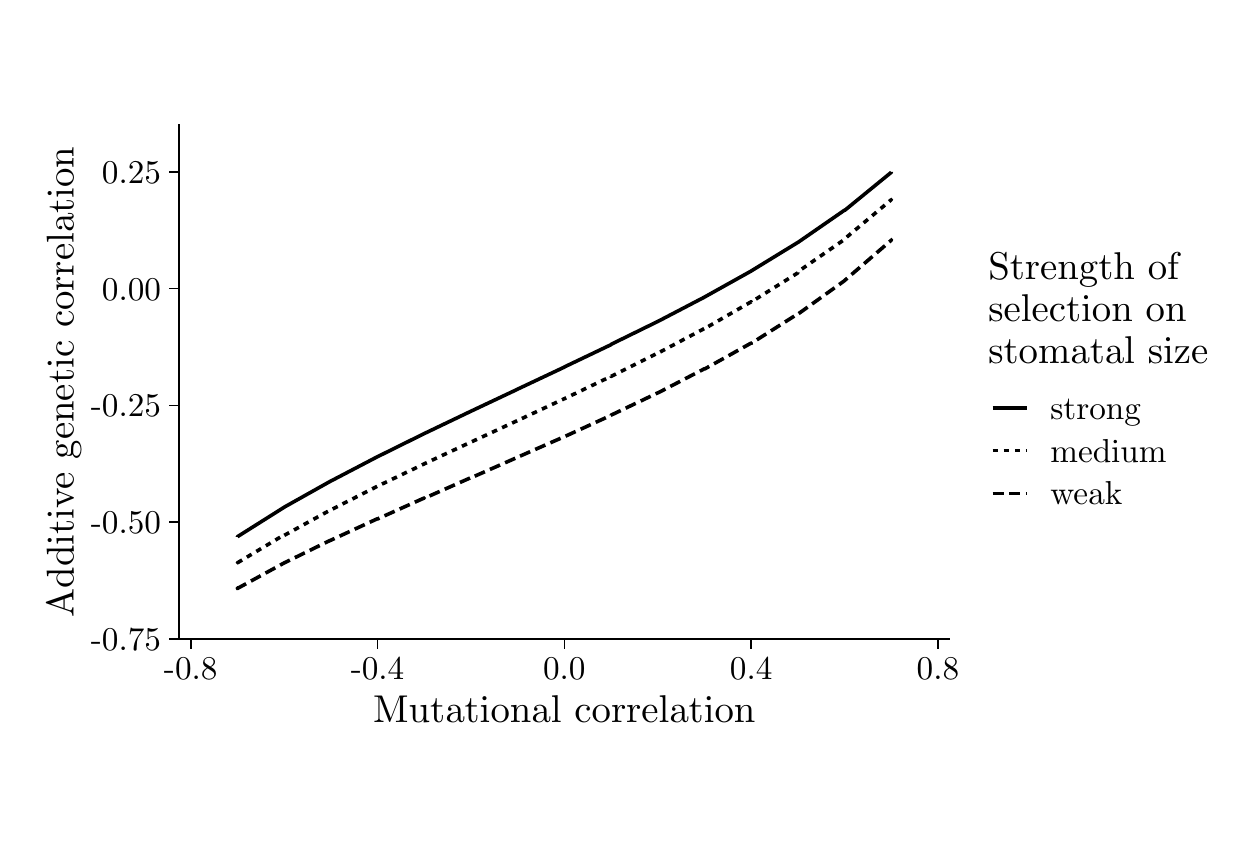
\begin{tikzpicture}[x=1pt,y=1pt]
\definecolor{fillColor}{RGB}{255,255,255}
\path[use as bounding box,fill=fillColor,fill opacity=0.00] (0,0) rectangle (433.62,289.08);
\begin{scope}
\path[clip] ( 54.69, 68.20) rectangle (333.15,253.84);
\definecolor{drawColor}{RGB}{0,0,0}

\path[draw=drawColor,line width= 1.3pt,line join=round] ( 75.79,105.11) --
	( 75.79,105.13) --
	( 75.79,105.14) --
	( 92.66,115.77) --
	( 92.66,115.79) --
	( 92.66,115.79) --
	(109.54,125.26) --
	(109.54,125.29) --
	(109.54,125.24) --
	(126.42,134.06) --
	(126.42,134.06) --
	(126.42,134.05) --
	(143.29,142.40) --
	(143.29,142.40) --
	(143.29,142.40) --
	(160.17,150.48) --
	(160.17,150.48) --
	(160.17,150.48) --
	(177.04,158.44) --
	(177.04,158.45) --
	(177.04,158.46) --
	(193.92,166.42) --
	(193.92,166.44) --
	(193.92,166.47) --
	(210.80,174.53) --
	(210.80,174.56) --
	(210.80,174.64) --
	(227.67,182.91) --
	(227.67,182.92) --
	(227.67,182.90) --
	(244.55,191.71) --
	(244.55,191.74) --
	(244.55,191.72) --
	(261.43,201.14) --
	(261.43,201.20) --
	(261.43,201.15) --
	(278.30,211.48) --
	(278.30,211.48) --
	(278.30,211.46) --
	(295.18,223.14) --
	(295.18,223.17) --
	(295.18,223.02) --
	(312.06,236.81) --
	(312.06,236.87) --
	(312.06,236.94);

\path[draw=drawColor,line width= 1.3pt,dash pattern=on 2pt off 2pt ,line join=round] ( 75.79, 95.71) --
	( 75.79, 95.70) --
	( 75.79, 95.71) --
	( 92.66,105.80) --
	( 92.66,105.82) --
	( 92.66,105.60) --
	(109.54,114.87) --
	(109.54,114.88) --
	(109.54,114.82) --
	(126.42,123.39) --
	(126.42,123.36) --
	(126.42,123.38) --
	(143.29,131.45) --
	(143.29,131.48) --
	(143.29,131.47) --
	(160.17,139.33) --
	(160.17,139.32) --
	(160.17,139.32) --
	(177.04,147.13) --
	(177.04,147.18) --
	(177.04,147.12) --
	(193.92,155.01) --
	(193.92,155.15) --
	(193.92,154.99) --
	(210.80,163.08) --
	(210.80,163.10) --
	(210.80,163.05) --
	(227.67,171.48) --
	(227.67,171.53) --
	(227.67,171.43) --
	(244.55,180.38) --
	(244.55,180.46) --
	(244.55,180.29) --
	(261.43,190.03) --
	(261.43,189.95) --
	(261.43,189.93) --
	(278.30,200.48) --
	(278.30,200.58) --
	(278.30,200.88) --
	(295.18,212.57) --
	(295.18,212.72) --
	(295.18,212.74) --
	(312.06,226.91) --
	(312.06,226.99) --
	(312.06,226.84);

\path[draw=drawColor,line width= 1.3pt,dash pattern=on 4pt off 2pt ,line join=round] ( 75.79, 86.47) --
	( 75.79, 86.67) --
	( 75.79, 86.44) --
	( 92.66, 95.65) --
	( 92.66, 95.67) --
	( 92.66, 95.66) --
	(109.54,103.91) --
	(109.54,103.90) --
	(109.54,103.87) --
	(126.42,111.66) --
	(126.42,111.67) --
	(126.42,111.55) --
	(143.29,119.13) --
	(143.29,119.15) --
	(143.29,119.01) --
	(160.17,126.49) --
	(160.17,126.52) --
	(160.17,126.40) --
	(177.04,133.86) --
	(177.04,133.92) --
	(177.04,133.87) --
	(193.92,141.29) --
	(193.92,141.28) --
	(193.92,141.27) --
	(210.80,149.00) --
	(210.80,149.00) --
	(210.80,149.06) --
	(227.67,157.11) --
	(227.67,157.10) --
	(227.67,157.07) --
	(244.55,165.83) --
	(244.55,165.75) --
	(244.55,165.70) --
	(261.43,175.11) --
	(261.43,175.15) --
	(261.43,174.98) --
	(278.30,185.67) --
	(278.30,185.67) --
	(278.30,185.55) --
	(295.18,197.66) --
	(295.18,197.81) --
	(295.18,197.70) --
	(312.06,212.27) --
	(312.06,212.52) --
	(312.06,212.47);
\end{scope}
\begin{scope}
\path[clip] (  0.00,  0.00) rectangle (433.62,289.08);
\definecolor{drawColor}{RGB}{0,0,0}

\path[draw=drawColor,line width= 0.6pt,line join=round,line cap=rect] ( 54.69, 68.20) --
	( 54.69,253.84);
\end{scope}
\begin{scope}
\path[clip] (  0.00,  0.00) rectangle (433.62,289.08);
\definecolor{drawColor}{RGB}{0,0,0}

\node[text=drawColor,anchor=base east,inner sep=0pt, outer sep=0pt, scale=  1.20] at ( 48.19, 64.07) {-0.75};

\node[text=drawColor,anchor=base east,inner sep=0pt, outer sep=0pt, scale=  1.20] at ( 48.19,106.26) {-0.50};

\node[text=drawColor,anchor=base east,inner sep=0pt, outer sep=0pt, scale=  1.20] at ( 48.19,148.45) {-0.25};

\node[text=drawColor,anchor=base east,inner sep=0pt, outer sep=0pt, scale=  1.20] at ( 48.19,190.64) {0.00};

\node[text=drawColor,anchor=base east,inner sep=0pt, outer sep=0pt, scale=  1.20] at ( 48.19,232.83) {0.25};
\end{scope}
\begin{scope}
\path[clip] (  0.00,  0.00) rectangle (433.62,289.08);
\definecolor{drawColor}{RGB}{0,0,0}

\path[draw=drawColor,line width= 0.6pt,line join=round] ( 51.19, 68.20) --
	( 54.69, 68.20);

\path[draw=drawColor,line width= 0.6pt,line join=round] ( 51.19,110.39) --
	( 54.69,110.39);

\path[draw=drawColor,line width= 0.6pt,line join=round] ( 51.19,152.58) --
	( 54.69,152.58);

\path[draw=drawColor,line width= 0.6pt,line join=round] ( 51.19,194.77) --
	( 54.69,194.77);

\path[draw=drawColor,line width= 0.6pt,line join=round] ( 51.19,236.96) --
	( 54.69,236.96);
\end{scope}
\begin{scope}
\path[clip] (  0.00,  0.00) rectangle (433.62,289.08);
\definecolor{drawColor}{RGB}{0,0,0}

\path[draw=drawColor,line width= 0.6pt,line join=round,line cap=rect] ( 54.69, 68.20) --
	(333.15, 68.20);
\end{scope}
\begin{scope}
\path[clip] (  0.00,  0.00) rectangle (433.62,289.08);
\definecolor{drawColor}{RGB}{0,0,0}

\path[draw=drawColor,line width= 0.6pt,line join=round] ( 58.91, 64.70) --
	( 58.91, 68.20);

\path[draw=drawColor,line width= 0.6pt,line join=round] (126.42, 64.70) --
	(126.42, 68.20);

\path[draw=drawColor,line width= 0.6pt,line join=round] (193.92, 64.70) --
	(193.92, 68.20);

\path[draw=drawColor,line width= 0.6pt,line join=round] (261.43, 64.70) --
	(261.43, 68.20);

\path[draw=drawColor,line width= 0.6pt,line join=round] (328.93, 64.70) --
	(328.93, 68.20);
\end{scope}
\begin{scope}
\path[clip] (  0.00,  0.00) rectangle (433.62,289.08);
\definecolor{drawColor}{RGB}{0,0,0}

\node[text=drawColor,anchor=base,inner sep=0pt, outer sep=0pt, scale=  1.20] at ( 58.91, 53.44) {-0.8};

\node[text=drawColor,anchor=base,inner sep=0pt, outer sep=0pt, scale=  1.20] at (126.42, 53.44) {-0.4};

\node[text=drawColor,anchor=base,inner sep=0pt, outer sep=0pt, scale=  1.20] at (193.92, 53.44) {0.0};

\node[text=drawColor,anchor=base,inner sep=0pt, outer sep=0pt, scale=  1.20] at (261.43, 53.44) {0.4};

\node[text=drawColor,anchor=base,inner sep=0pt, outer sep=0pt, scale=  1.20] at (328.93, 53.44) {0.8};
\end{scope}
\begin{scope}
\path[clip] (  0.00,  0.00) rectangle (433.62,289.08);
\definecolor{drawColor}{RGB}{0,0,0}

\node[text=drawColor,anchor=base,inner sep=0pt, outer sep=0pt, scale=  1.40] at (193.92, 37.96) {Mutational correlation};
\end{scope}
\begin{scope}
\path[clip] (  0.00,  0.00) rectangle (433.62,289.08);
\definecolor{drawColor}{RGB}{0,0,0}

\node[text=drawColor,rotate= 90.00,anchor=base,inner sep=0pt, outer sep=0pt, scale=  1.40] at ( 16.64,161.02) {Additive genetic correlation};
\end{scope}
\begin{scope}
\path[clip] (  0.00,  0.00) rectangle (433.62,289.08);
\definecolor{drawColor}{RGB}{0,0,0}

\node[text=drawColor,anchor=base west,inner sep=0pt, outer sep=0pt, scale=  1.40] at (347.15,197.92) {Strength of};

\node[text=drawColor,anchor=base west,inner sep=0pt, outer sep=0pt, scale=  1.40] at (347.15,182.80) {selection on};

\node[text=drawColor,anchor=base west,inner sep=0pt, outer sep=0pt, scale=  1.40] at (347.15,167.68) {stomatal size};
\end{scope}
\begin{scope}
\path[clip] (  0.00,  0.00) rectangle (433.62,289.08);
\definecolor{drawColor}{RGB}{0,0,0}

\path[draw=drawColor,line width= 1.3pt,line join=round] (348.69,151.62) -- (361.01,151.62);
\end{scope}
\begin{scope}
\path[clip] (  0.00,  0.00) rectangle (433.62,289.08);
\definecolor{drawColor}{RGB}{0,0,0}

\path[draw=drawColor,line width= 1.3pt,dash pattern=on 2pt off 2pt ,line join=round] (348.69,136.22) -- (361.01,136.22);
\end{scope}
\begin{scope}
\path[clip] (  0.00,  0.00) rectangle (433.62,289.08);
\definecolor{drawColor}{RGB}{0,0,0}

\path[draw=drawColor,line width= 1.3pt,dash pattern=on 4pt off 2pt ,line join=round] (348.69,120.82) -- (361.01,120.82);
\end{scope}
\begin{scope}
\path[clip] (  0.00,  0.00) rectangle (433.62,289.08);
\definecolor{drawColor}{RGB}{0,0,0}

\node[text=drawColor,anchor=base west,inner sep=0pt, outer sep=0pt, scale=  1.20] at (369.55,147.49) {strong};
\end{scope}
\begin{scope}
\path[clip] (  0.00,  0.00) rectangle (433.62,289.08);
\definecolor{drawColor}{RGB}{0,0,0}

\node[text=drawColor,anchor=base west,inner sep=0pt, outer sep=0pt, scale=  1.20] at (369.55,132.09) {medium};
\end{scope}
\begin{scope}
\path[clip] (  0.00,  0.00) rectangle (433.62,289.08);
\definecolor{drawColor}{RGB}{0,0,0}

\node[text=drawColor,anchor=base west,inner sep=0pt, outer sep=0pt, scale=  1.20] at (369.55,116.69) {weak};
\end{scope}
\end{tikzpicture}
